\chapter{Results and Analysis}
\label{sec:rna}

% TODO: Include mention that this spans across 17 and 18 data.

Each of the GAN models described in Section \ref{sec:model_arch} were used to create artificial NIDS alert data.  Using the methods described in Section \ref{sec:meth} the fidelity of the learned model was analyzed. This analysis can be broken down into the following sections:

\begin{enumerate}
	\item Thorough Hyperparameter Search - Individual hyperparameters were tuned for each model to see their impact on histogram intersection. Top candidate values were selected for a full hyperparameter search where all combinations of hyperparameter values. The results are presented for both WGAN-GP and the improved WGAN-GPMI.

	\item Alert Fidelity - A subset of target IPs from both the CPTC'17 and CPTC'18 dataset were used for training WGAN-GP and WGAN-GPMI models. The results of these models were analyzed and visualized using histogram intersection and Jensen-Shannon Divergence.

	\item Alert Dependency - For the same subset of target IPs alert dependencies were identified by using drop in histogram intersection, entropy computation, and conditional probability tables.

	\item Output Modes Captured - The number of output modes captured by the model is comprised of two components. How many of the true output modes are output by the model. And how many output modes by the model do not occur in the ground truth.

\end{enumerate}

The CPTC'17 dataset was segmented on per-target IP basis and used across all experiments. For the hyper parameter search the IP which contained the most alerts, 10.0.0.100, was used. For the following experiments on alert fidelity, modeling dependency, and output modes captured the following four IP's were used: \{10.0.0.100, 10.0.0.22, 10.0.0.27, 10.0.99.143\}. These four IP addresses provided a mixture of Windows and Linux Machines, with varying purpose, and contained the 4 greatest counts of alerts. Table. \ref{tab:mapping} summarizes the differences between each of these machines.

\begin{table}[!htbp]
	\caption{Mapping of Target IP Address to Machine Usage/Purpose}
	\label{table:mapping}
	\centering
	\begin{tabular}{c|c|c|c}
		\textbf{IP Address} & \textbf{Operating System} & \textbf{Machine Usage} & \textbf{Number of Alerts}\\
		\hline
		10.0.0.100 & Windows & Active Directory Server & 3388\\
		\hline
		10.0.0.27 & Ubuntu & HTTP Server & 3166\\
		\hline
		10.0.0.22 & Ubuntu & MySQL Server & 2974\\
		\hline
		10.0.99.143 & Ubuntu & HTTP Server & 2182
	\end{tabular}
\end{table}

It was important to consider the machines with the greatest number of alerts as Deep Learning, especially for GANs, requires very large datasets.

\section{Thorough Hyperparameter Search}
\label{sec:search}
A two part hyperparameter search was employed to find optimal values for generating alerts from the CTPC datasets. First, individual parameters were tested in order to find several values which resulted in promising results. For each parameter value tested, the histogram intersection was computed for all possible feature value combinations. These values were then plotted against all other parameter settings results for WGAN-GP and WGAN-GPMI. Then, these values were taken and used for a full parameter sweep, which tested every possible combination of the parameter values available. Several candidate values were selected for each of the hyperparameters due to the unknown nature of hyperparameter interaction.

This two stage search was carried out twice, once for each of the GAN models presented in Section \ref{sec:model_arch}. The parameters tested included lambda, batch size, learning rate, hidden dimension, and number of epochs.

\subsection{Lambda}
\label{sec:lam}
The lambda parameter was used as a coefficient to the gradient penalty term applied to the discriminator. The values tested for lambda were $\{0.05, 0.1, 0.2, 0.3, 0.4\}$. The intersection vs. parameter setting plots for WGAN-GP and WGAN-GPMI may be seen in Fig. \ref{fig:wgan_lam} and Fig. \ref{fig:gpmi_lam} respectively.

\begin{figure}[!htbp]
	\centering

	\begin{subfigure}{.7\textwidth}
		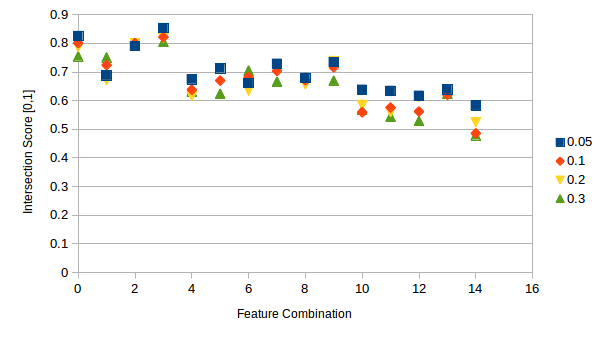
\includegraphics[width=\textwidth]{wgan_lam}
	\end{subfigure}%
	\begin{subfigure}{.3\textwidth}
		\caption{
			All other hyperparameters were held constant at the following values: $epochs=180$, $batch\_size = 100$, $learning\_rate=5e-5$, $hidden\_dimension=128$
		}
		\label{fig:wgan_lam}
	\end{subfigure}%

	\begin{subfigure}{.7\textwidth}
		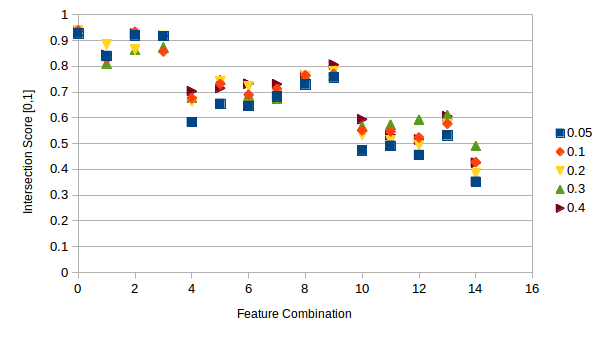
\includegraphics[width=\textwidth]{gpmi_lam}
	\end{subfigure}%
	\begin{subfigure}{.3\textwidth}
		\caption{
			All other hyperparameters were held constant at the following values: $epochs=250$, $batch\_size=100$, $learning\_rate=5e-4$, $hidden\_dimension=128$
		}
		\label{fig:gpmi_lam}
	\end{subfigure}%
	\caption{Lambda Parameter Search}
\end{figure}

The performance of all the values tested was very close. For the WGAN-GP model smaller values such as $\{0.05, 0.1, 0.2\}$ performed well. In the WGAN-GPMI model the larger values tested, $\{0.2,0.3,0.4\}$ performed well. This suggests that the WGAN-GPMI model requires stronger enforcement of the gradient penalty than the WGAN-GP model does. Given that the gradient of the generator is changed from an outside source (the mutual information estimate) in addition to the discriminator feedback, the discriminator may be trying to make larger gradient changes to identify generated samples.


\subsection{Batch Size}
\label{sec:bs}

The batch size determines how many alert samples were fed into the model in parallel. Higher batch sizes can are more computationally intensive, but provide a better representation of the ground truth data distribution. Additionally, larger batch sizes reduce the number of steps required to complete a full epoch of training.

The values tested for batch size were $\{10, 25, 50, 100, 150, 250, 500, 1000\}$. The intersection vs. parameter setting plots for WGAN-GP and WGAN-GPMI may be seen in Fig. \ref{fig:wgan_batch_size} and Fig. \ref{fig:gpmi_batch_size} respectively.

\begin{figure}[!htbp]
	\centering
	\begin{subfigure}{.7\textwidth}
		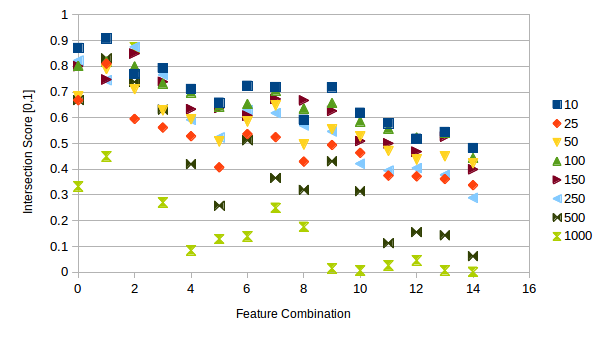
\includegraphics[width=\textwidth]{wgan_batch_size}
	\end{subfigure}%
	\begin{subfigure}{.3\textwidth}
		\caption{
			All other hyperparameters were held constant at the following values: $epochs=180$, $learning\_rate=5e-5$, $hidden\_dimension=128$, $\lambda=0.1$
		}
		\label{fig:wgan_batch_size}
	\end{subfigure}%

	\begin{subfigure}{.7\textwidth}
		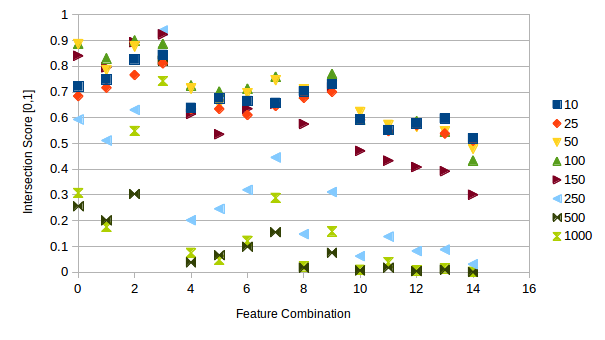
\includegraphics[width=\textwidth]{gpmi_batch_size}
	\end{subfigure}%
	\begin{subfigure}{.3\textwidth}
		\caption{
			All other hyperparameters were held constant at the following values: $epochs=250$, $learning\_rate=5e-4$, $hidden\_dimension=128$, $\lambda=0.3$
		}
		\label{fig:gpmi_batch_size}
	\end{subfigure}%
	\caption{Batch Size Parameter Search}
\end{figure}

The overall range and trends of intersection scores are very similar for both WGAN-GP and WGAN-GPMI. It is interesting to observe that for the WGAN-GPMI model that the performance drop after using batch sizes greater than 250 is much greater than that of the WGAN-GP model. Regardless, the top selections for the full parameter search are $\{10,25,50,100,150\}$ for the WGAN model and $\{50,100\}$ for the WGAN-GPMI model.

\subsection{Learning Rate}
\label{sec:lr}

The learning rate of the optimizer defines the base step size, weighted by the gradient of the loss, that is taken when adjusting parameter weights during training. A large learning rate converges quickly, but may overshoot the global optimum and never reach peak performance. A small learning rate won't overshoot the global optimum, however will take significantly longer to converge. Due to the categorical output of alert data and existing difficulty in optimizing GANs, small learning rates were tested. This allowed the network to be able to make fine tuned changes to network weights. Additionally, the ADAM optimizer was used, allowing for weight decay over time to modify the learning rate parameter.


The values tested for learning rate were $\{1e-5, 5e-5, 1e-4, 5e-4, 1e-3\}$. The intersection vs. parameter setting plots for WGAN-GP and WGAN-GPMI may be seen in Fig. \ref{fig:wgan_lr} and Fig. \ref{fig:gpmi_lr} respectively.

\begin{figure}[!htbp]
	\centering
	\begin{subfigure}{.7\textwidth}
		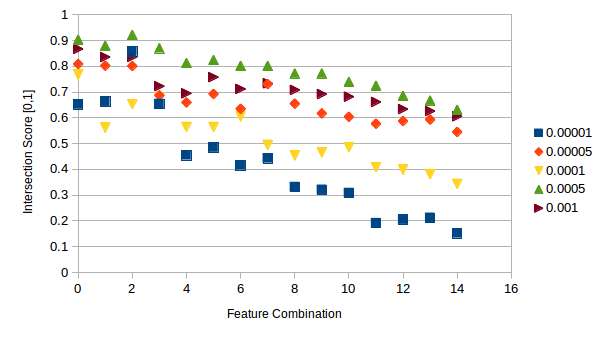
\includegraphics[width=\textwidth]{wgan_lr}
	\end{subfigure}%
	\begin{subfigure}{.3\textwidth}
		\caption{
			All other hyperparameters were held constant at the following values: $epochs=180$, $batch\_size = 100$, $hidden\_dimension=128$, $\lambda=0.1$
		}
		\label{fig:wgan_lr}
	\end{subfigure}%

	\begin{subfigure}{.7\textwidth}
		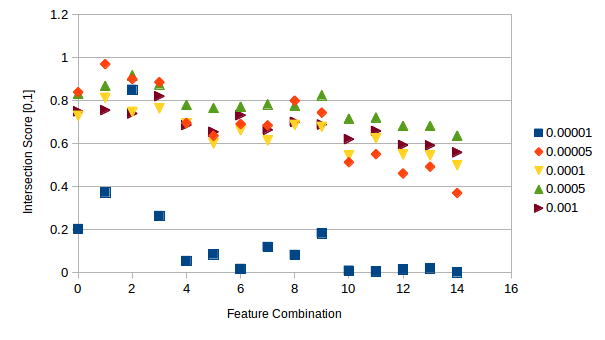
\includegraphics[width=\textwidth]{gpmi_lr}
	\end{subfigure}%
	\begin{subfigure}{.3\textwidth}
		\caption{
			All other hyperparameters were held constant at the following values: $epochs=250$, $batch\_size=100$, $hidden\_dimension=128$, $\lambda=0.3$
		}
		\label{fig:gpmi_lr}
	\end{subfigure}%
	\caption{Learning Rate Parameter Search}
\end{figure}

For both of the models tested, the smallest learning rate $1e-5$ performs poorly. Interestingly, in the WGAN-GP model the subsequent three learning rates $\{5e-5,1e-4,5e-4\}$ oscillate between performing well and poorly. due to this oscillations $1e-4$ is dropped, leaving $\{5e-5,5e-4,1e-3\}$ for the full parameter search. For the WGAN-GPMI model $\{1e-4, 5e-4, 1e-3\}$ are all used in the full parameter test.


\subsection{Hidden Dimension}
\label{sec:hdim}

The hidden dimension size determines the number of hidden units available in each hidden layer. Higher hidden dimensions provide more learnable connections to the network allowing the network to complex approximations. On the other hand, larger hidden dimension sizes leads to potential overfitting and raises the computational complexity of training the network.

The values tested for hidden dimension were $\{64, 128, 256, 384, 512\}$. The intersection vs. parameter setting plots for WGAN-GP and WGAN-GPMI may be seen in Fig. \ref{fig:wgan_hdim} and Fig. \ref{fig:gpmi_hdim} respectively.

\begin{figure}[!htbp]
	\centering
	\begin{subfigure}{.7\textwidth}
		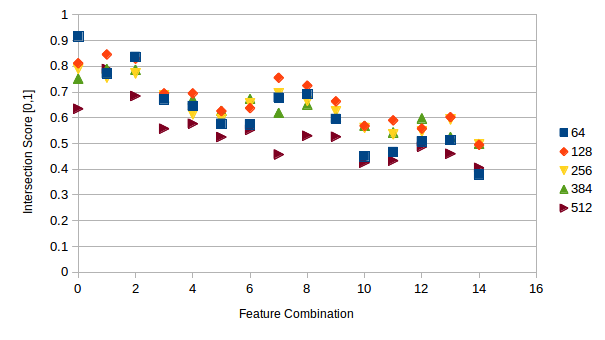
\includegraphics[width=\textwidth]{wgan_hdim}
	\end{subfigure}%
	\begin{subfigure}{.3\textwidth}
		\caption{
			All other hyperparameters were held constant at the following values: $epochs=180$, $batch\_size = 100$, $learning\_rate=5e-5$, $\lambda=0.1$
		}
		\label{fig:wgan_hdim}
	\end{subfigure}%

	\begin{subfigure}{.7\textwidth}
		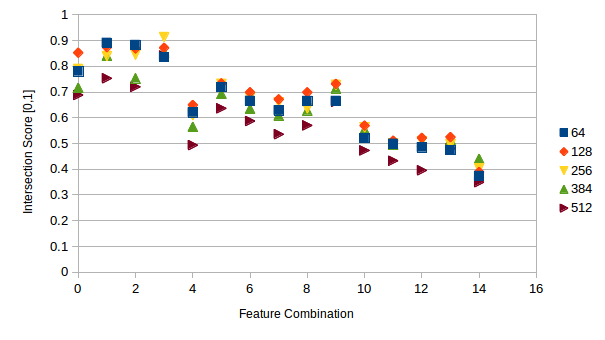
\includegraphics[width=\textwidth]{gpmi_hdim}
	\end{subfigure}%
	\begin{subfigure}{.3\textwidth}
		\caption{
			All other hyperparameters were held constant at the following values: $epochs=250$, $batch\_size=100$, $learning\_rate=5e-4$, $\lambda=0.3$
		}
		\label{fig:gpmi_hdim}
	\end{subfigure}%
	\caption{Hidden Dimension Parameter Search}
\end{figure}


The range of histogram intersection scores for the hidden parameter search is far smaller than the other hyperparameters. For the WGAN-GP model $\{128, 256, 384\}$ had the highest intersection scores, while $\{64,128,256\}$ performed well for the WGAN-GPMI model.


\subsection{Epochs}
\label{sec:epoch}

The number of epochs determined how many times the network was exposed to the full dataset during training. Using a large number of epochs allows for the network to get more exposure to the ground truth distribution. However using a very large number of epochs can lead to the network memorizing the data.

Due to the small size of the CPTC dataset, large values for epochs were tested. These values included $\{50, 100, 150, 200, 250\}$. The intersection vs. parameter setting plots for WGAN-GP and WGAN-GPMI may be seen in Fig. \ref{fig:wgan_epoch} and Fig. \ref{fig:gpmi_epoch} respectively.

\begin{figure}[!htbp]
	\centering
	\begin{subfigure}{.7\textwidth}
		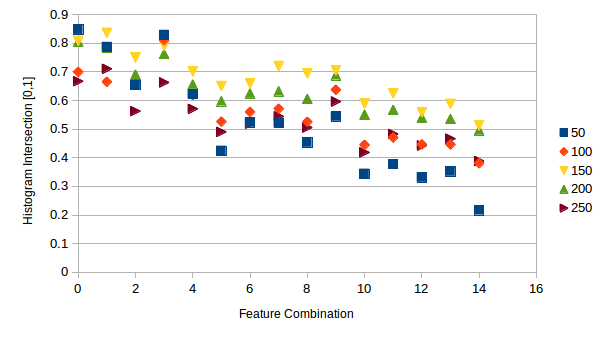
\includegraphics[width=\textwidth]{wgan_epoch}
	\end{subfigure}%
	\begin{subfigure}{.3\textwidth}
		\caption{
			All other hyperparameters were held constant at the following values: $batch\_size = 100$, $learning\_rate=5e-5$, $hidden\_dimension=128$, $\lambda=0.1$
		}
		\label{fig:wgan_epoch}
	\end{subfigure}%

	\begin{subfigure}{.7\textwidth}
		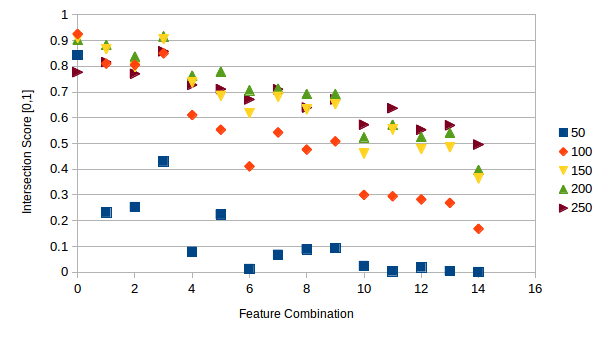
\includegraphics[width=\textwidth]{gpmi_epoch}
	\end{subfigure}%
	\begin{subfigure}{.3\textwidth}
		\caption{
			All other hyperparameters were held constant at the following values: $batch\_size=100$, $learning\_rate=5e-4$, $hidden\_dimension=128$, $\lambda=0.3$
		}
		\label{fig:gpmi_epoch}
	\end{subfigure}%
	\caption{Epochs Parameter Search}
\end{figure}

Increasing the number of epochs is critical for the WGAN-GPMI model to perform well. This makes intuitive sense, as this model requires the optimization of three neural networks. The $30$ epochs test case highlights this, as nearly all 3-tuple and 4-tuple feature combinations have 0 intersection with the ground truth distribution. Comparatively, the WGAN-GP model is able to achieve results within the range of $20-30$ percent; still the worst result of the values tested, but significantly better than WGAN-GPMI. For the WGAN-GP model, $\{100,150,200\}$ epochs were selected for the full hyperparameter sweep. For the WGAN-GPMI model, $\{150, 200, 250\}$ were selected.

\subsection{Full Parameter Sweep}

Collecting the candidate values from Sections \ref{sec:lam} through \ref{sec:epoch}, a full parameter search was carried out to test all combinations of these values. The values under test for each model may be seen in Table \ref{tab:param_sweep}, along with the unique number of combinations tested.

\begin{table}[!htbp]
	\centering
	\caption{Candidate Parameters for WGAN-GP and WGAN-GPMI}
	\label{tab:param_sweep}
	\begin{tabular}{l|ccccc|l|cccl}
		\cline{1-11}
		\multicolumn{6}{c}{\textbf{WGAN-GP Parameters}} & \multicolumn{1}{l}{} & \multicolumn{4}{c}{\textbf{WGAN-GPMI Parameters}} \\
		\cline{1-11}
		Lambda & 0.05 & 0.1 & 0.2 & & & & 0.2 & 0.3 & 0.4 & \\
		Batch Size & 10 & 25 & 50 & 100 & 150 & & 50 & 100 &  & \\
		Learning Rate & 5e-5 & 5e-4 & 1e-3 & & & & 5e-5 & 1e-4 & 5e-4 & 1e-3 \\
		Hidden Dimension & 128 & 256 & 384 & & & & 64 & 128 & 256 & \\
		Epochs & 100 & 150 & 200 & & & & 150 & 200 & 250 & \\
		\cline{1-11}
		\multicolumn{3}{l|}{Number of Unique Combinations} & \multicolumn{3}{c}{405} & \multicolumn{1}{|l|}{} & \multicolumn{4}{c}{216} \\ \cline{1-11}
	\end{tabular}
\end{table}

Given the scale of the combinations tested a simple 3 step heuristic was defined to identify the combinations which performed well. For each unique combination of features:
\begin{enumerate}
	\item The highest intersection score achieved was highlighted in yellow.
	\item Intersection scores that fell within the 90th percentile were highlighted in green
	\item Intersection scores that fell within the 80th percentile were highlighted in red.
\end{enumerate}

This system reduced the search of possible combinations, and allowed for quick visual identification of values which performed well. Identifying the highest intersection score per feature combination is not sufficient criteria to identify the best hyperparameter combination as scores are very close and can be noisy. Adding in the $90^{th}$ constraint helps to identify other candidates with high performing intersection scores. Finally, the $80^{th}$ percentile constraint is meant to act as a lower bound as values which fall within in it are still good, and values which are not highlighted at all should raise questions about model performance. For example, if the individual feature intersections are within the $90^{th}$ percentile but 3-tuple and 4-tuple combinations are completely not highlighted, the model may have failed to capture high order dependencies in the distribution of the data. Thus, that parameter setting should not be considered for use in future experiments.

A subsection of the highlighted table for the WGAN-GP model is given in Fig. \ref{fig:highlighted_param_wgan}. Note that the row with the red arrow pointing to it performs well, as 6 of it's 15 values are the highest performing intersection scores with an additional 6 in the $90^{th}$ percentile.

\begin{figure}[!htbp]
	\centering
	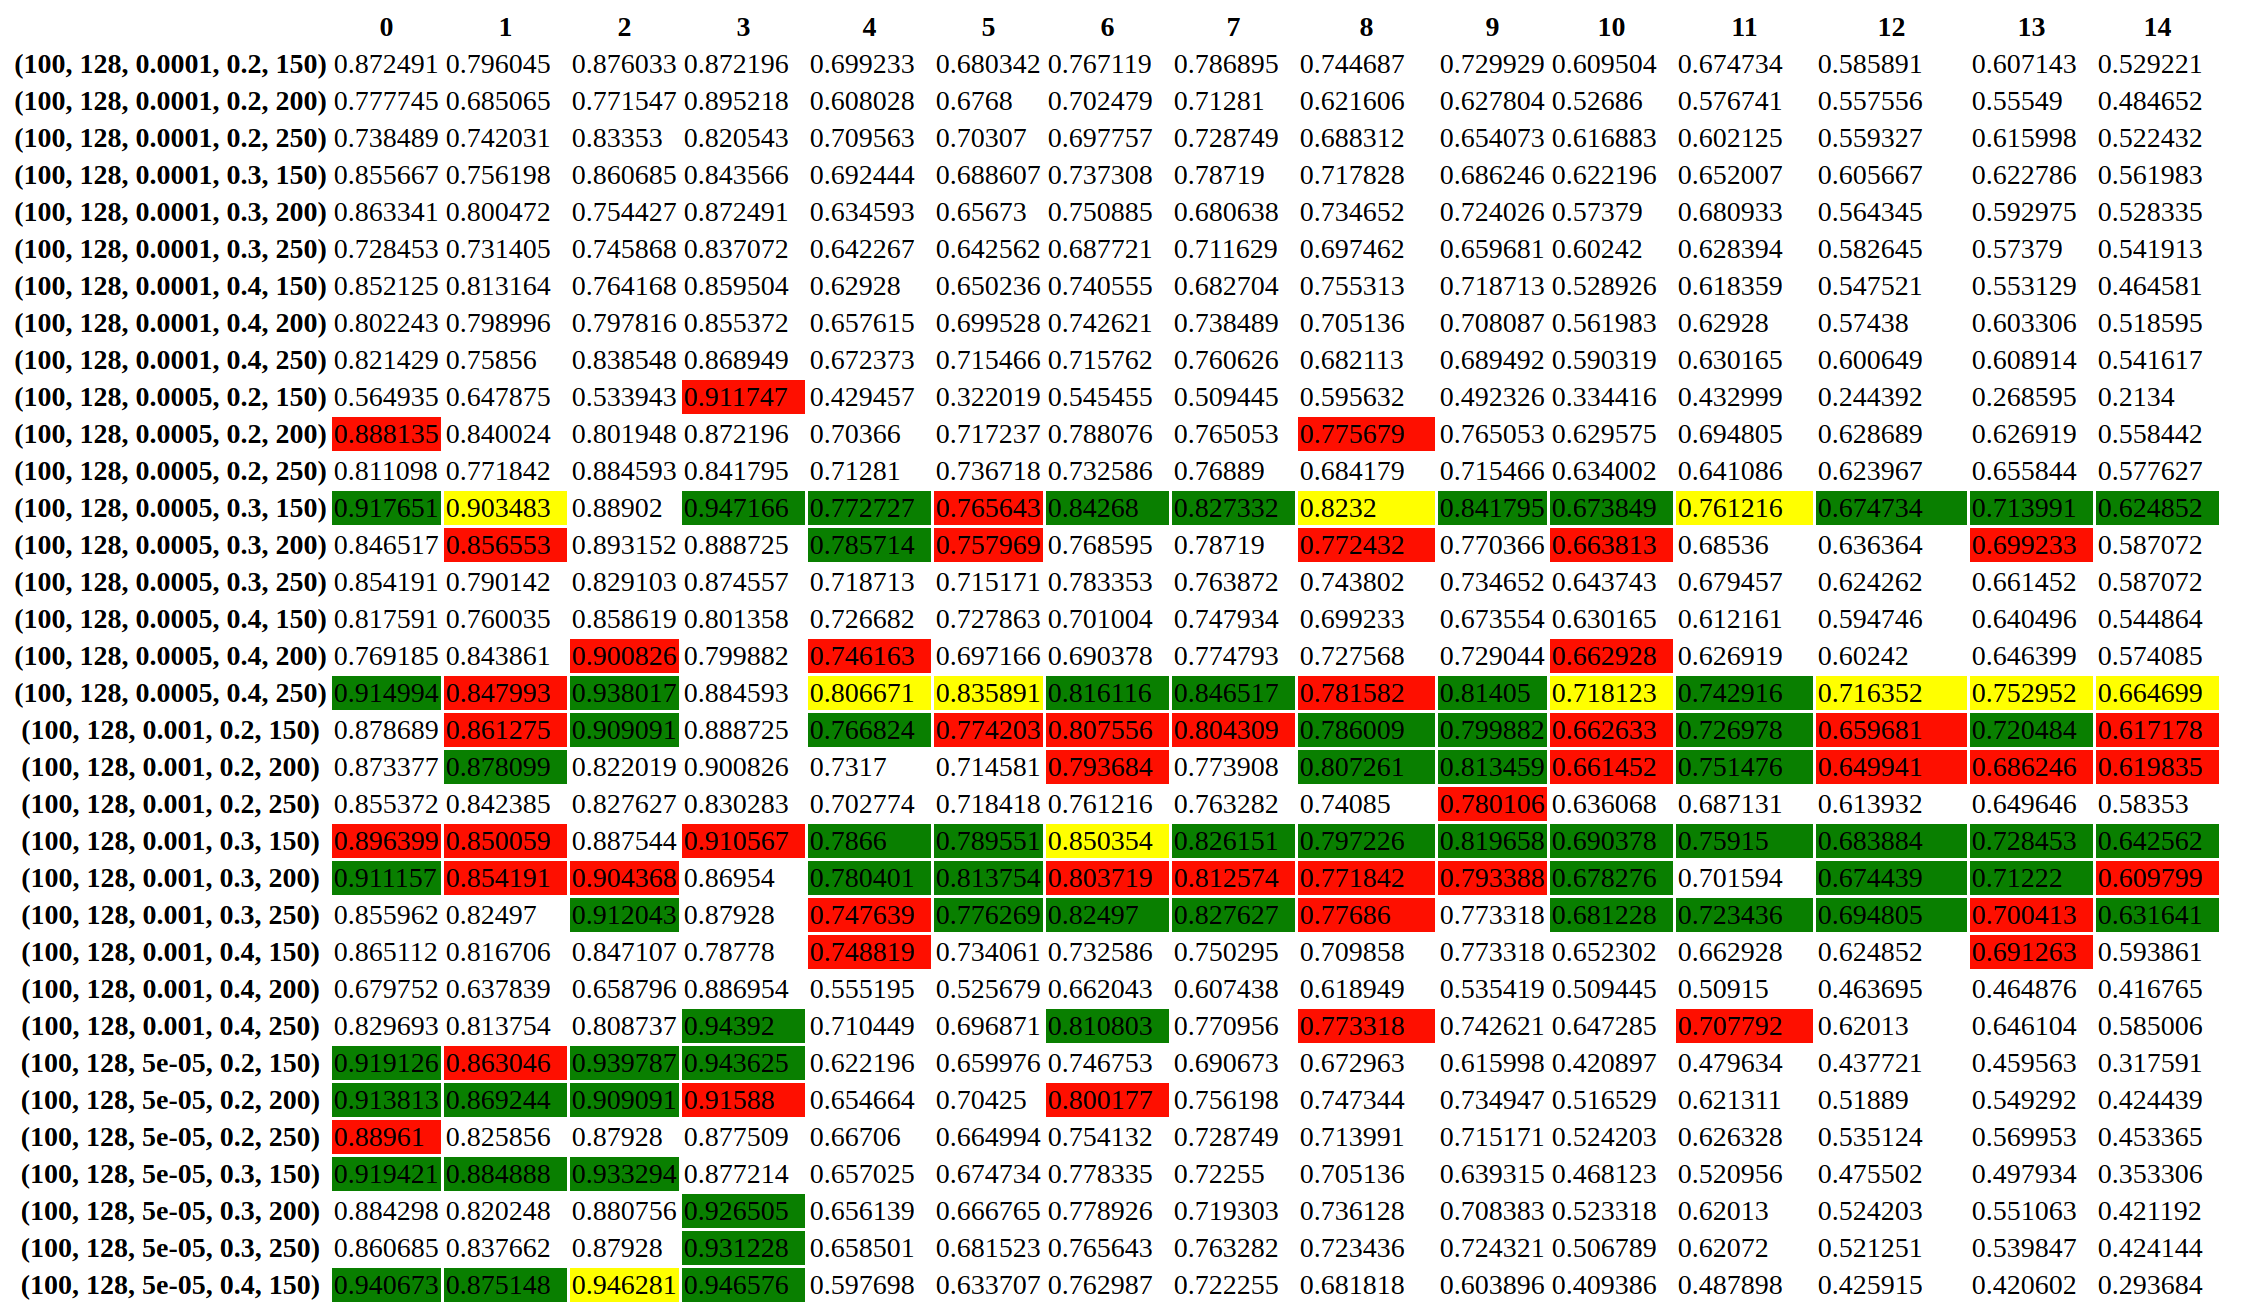
\includegraphics[width=\textheight,height=\textwidth,angle=90]{gpmi_full_param_search}
	\caption{
		Subsection of WGAN-GP Hyperparameter Search Results
	}
	\label{fig:highlighted_param_wgan}
\end{figure}

Similarly, a subsection of the highlighted table for the WGAN-GPMI model is given in Fig. \ref{fig:highlighted_param_gpmi}. Note that the row with the red arrow pointing to it performs well, as 6 of it's 15 values are the highest performing intersection scores with an additional 6 in the $90^{th}$ percentile.

\begin{figure}[!htbp]
	\centering
	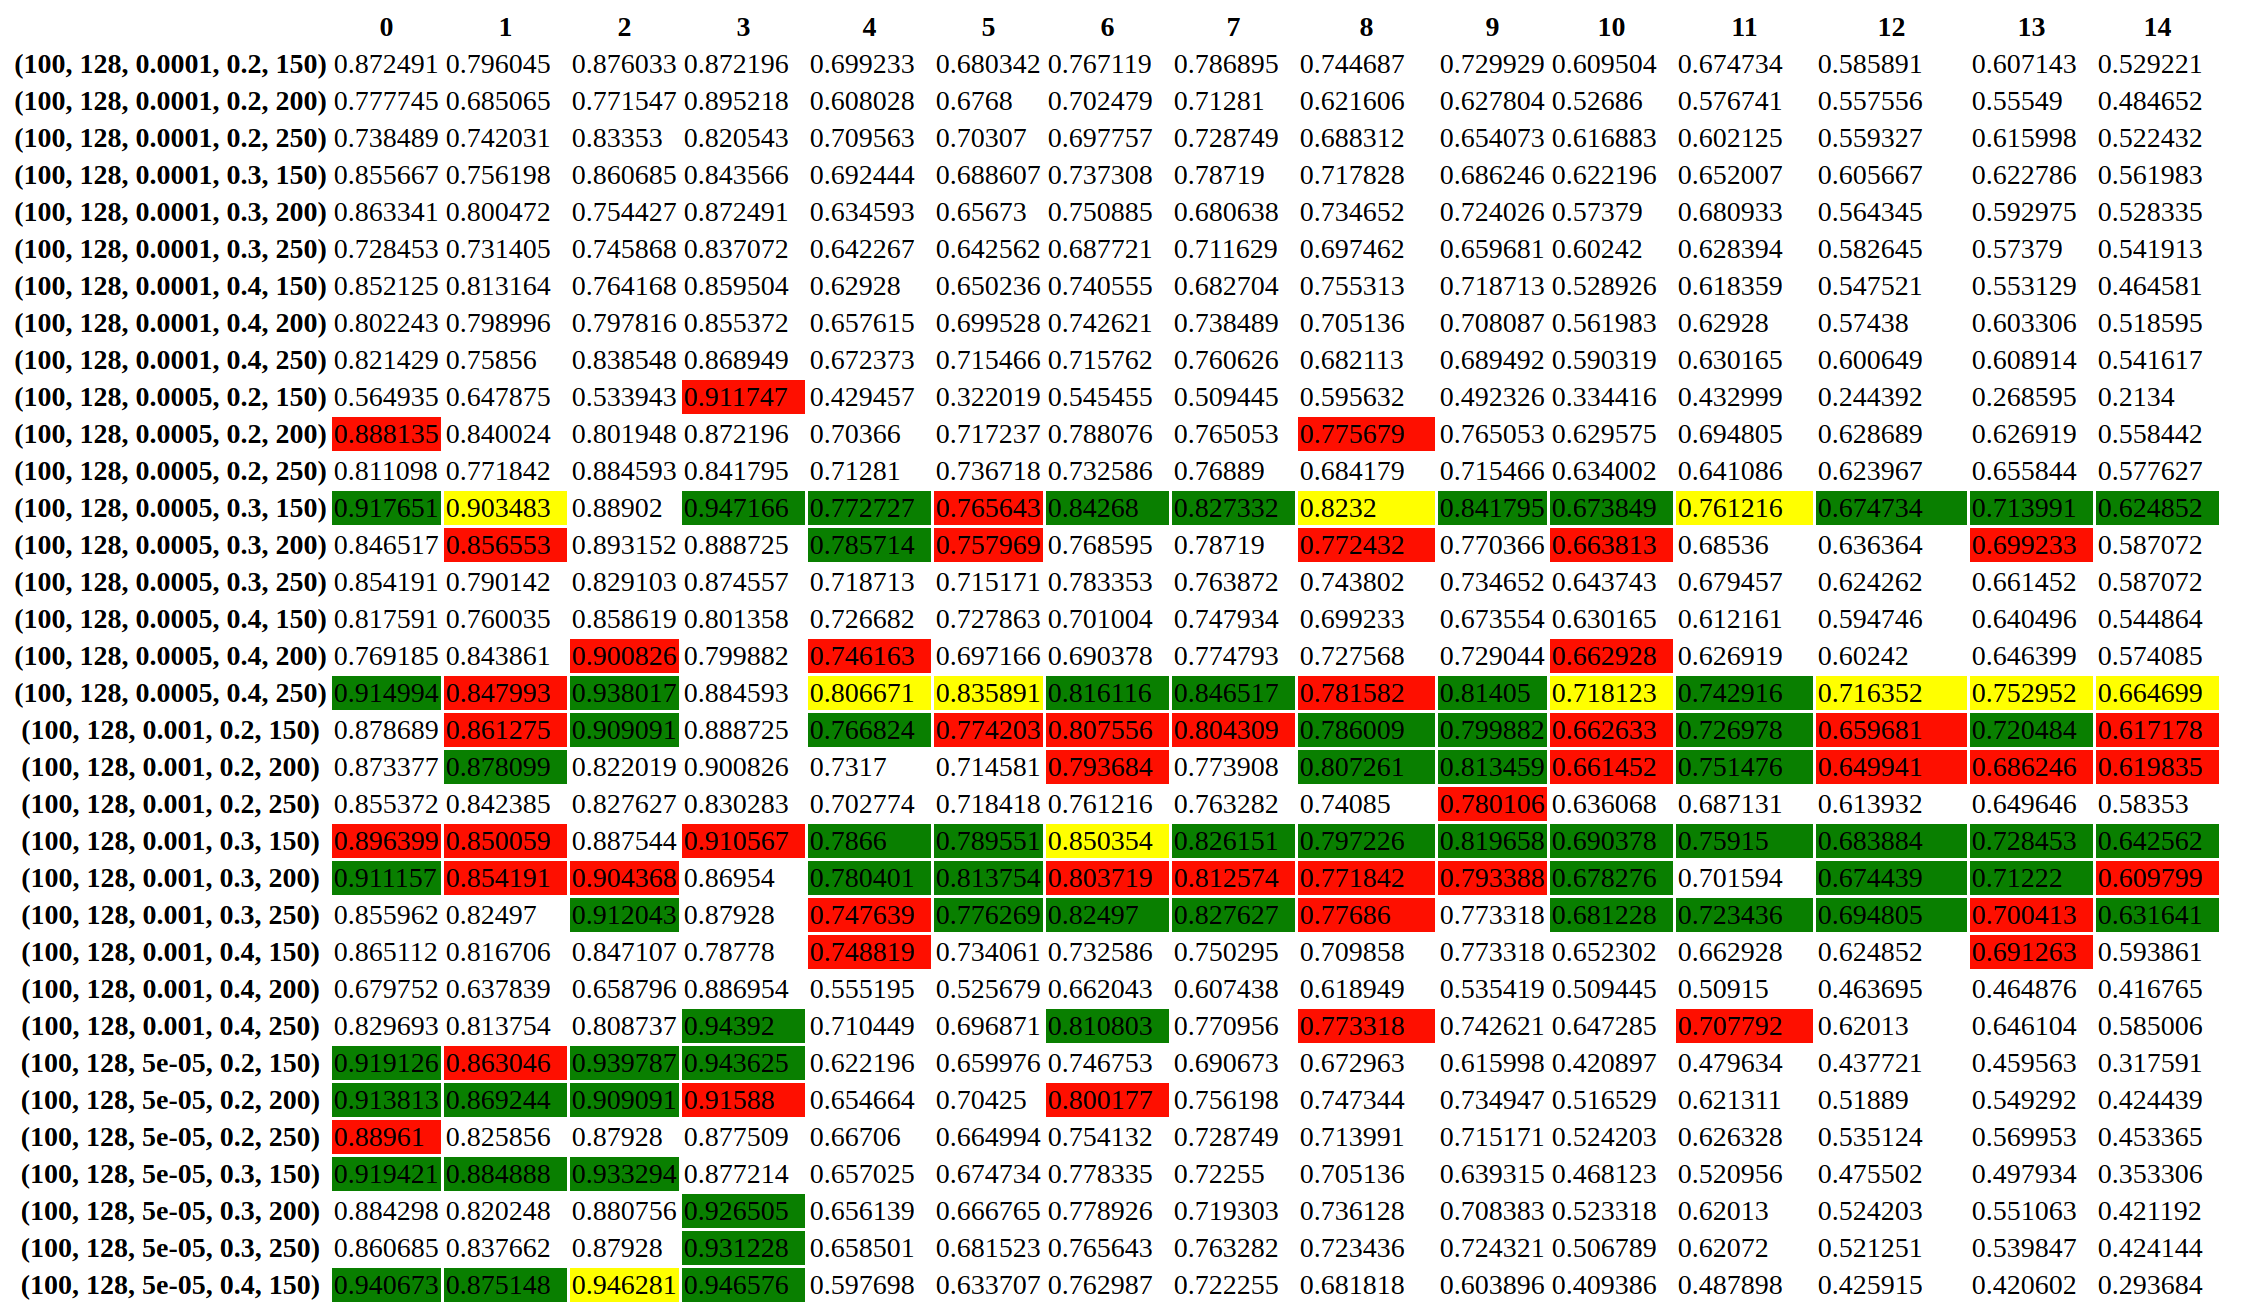
\includegraphics[width=\textheight,height=\textwidth,angle=90]{gpmi_full_param_search}
	\caption{
		Subsection of WGAN-GPMI Hyperparameter Search Results
	}
	\label{fig:highlighted_param_gpmi}
\end{figure}


\section{Alert Fidelity}
\label{sec:fidel}

Two metrics were employed in order to identify the fidelity of alert generation. Each metric was scaled such that it could be used to analyze individual feature performance as well as n-tuple combinations of features. This allowed for both low and high level performance of the model to be assessed. These metrics were the Histogram Intersection and Jensen Shannon Divergence.

\subsection{Histogram Intersection}
\label{sec:inter}

The histogram intersection was computed for all feature combinations across all 4 IPs tested. For each IP, all possible combinations of features were analyzed. This resulted in 4 intersections representing the individual features, 6 representing pairs of features, 4 representing 3-tuples, and a single histogram representing 4-tuple combinations.

Fig. \ref{fig:inter} steps through these levels of combinations for target 10.0.0.100. The top left plot shows the intersection of timebins. The top right plot shows the histogram combination of timebin and destination port category. The bottom right adds the alert signature feature to the histogram. And finally, the bottom right shows all 4 features under test as a single joint histogram. It is important to note that as the number of features considered in the combination increases so does the complexity of recreating the data with high fidelity; individual occurrences of features drops, while the number of unique features to output rises.


\begin{figure}[!htbp]
	\centering
	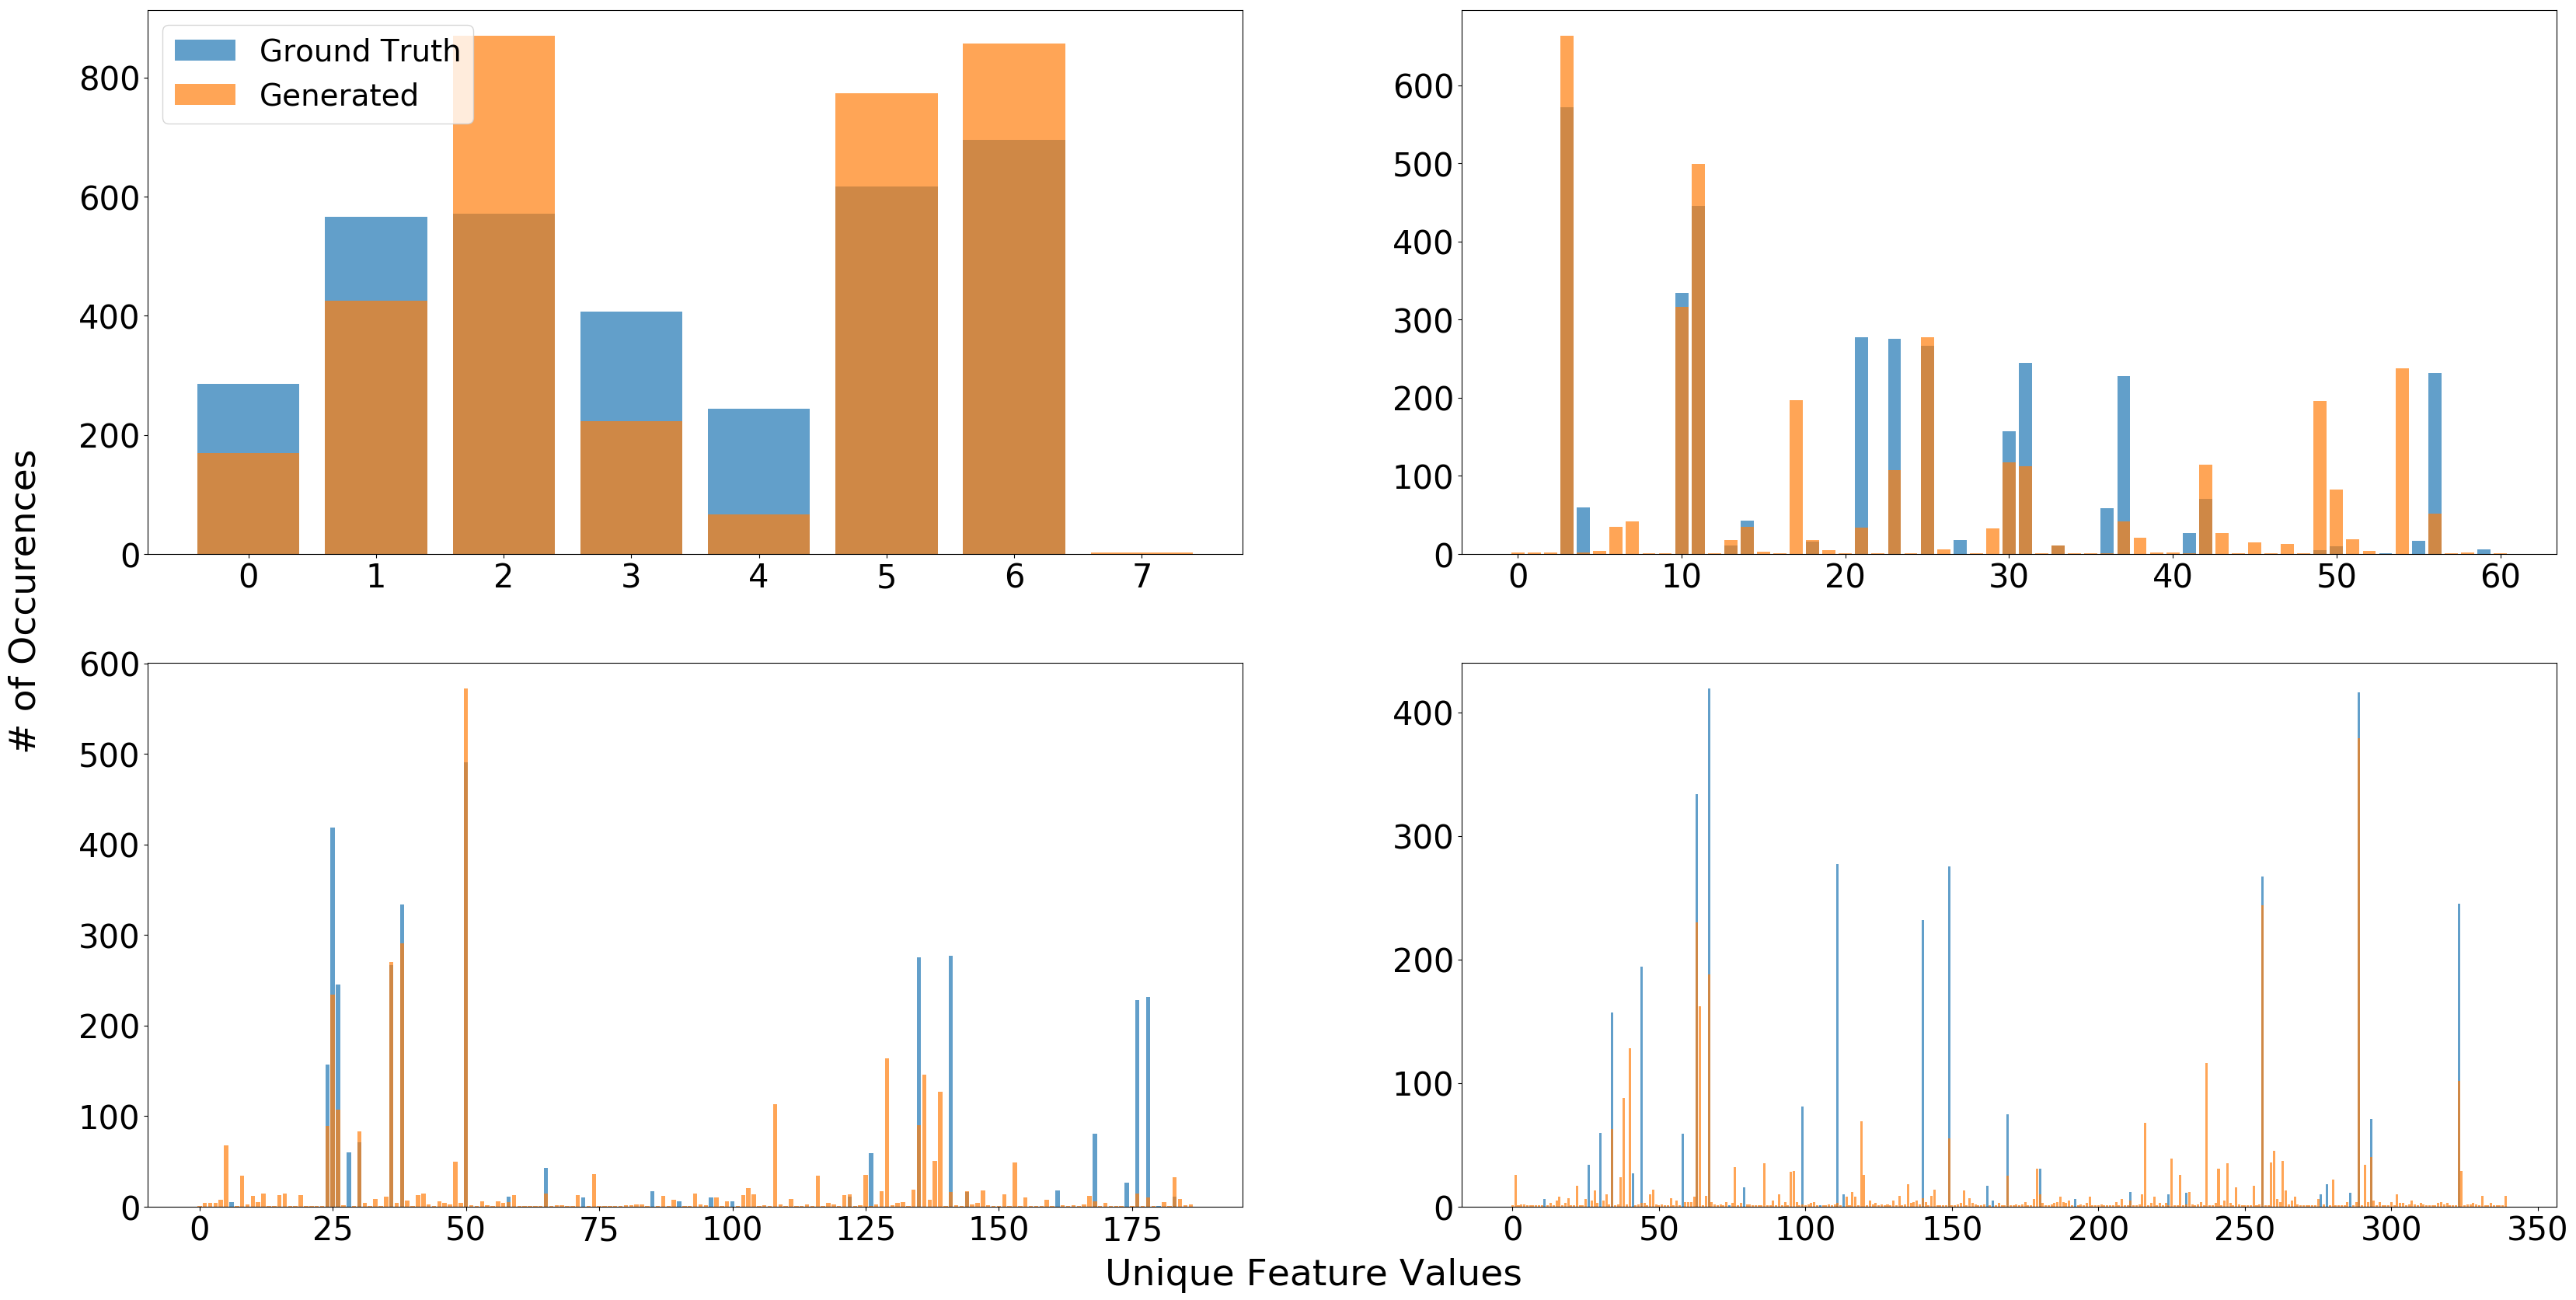
\includegraphics[width=\textwidth]{10_0_0_100_inter_gpmi}
	\caption{
		WGAN-GPMI Intersection of Histograms Across All N-Tuples
	}
	\label{fig:inter}
\end{figure}

The histogram intersection was used to analyze the fidelity of results from both of the models tested. In general, the WGAN-GPMI is able to outperform the standard WGAN-GP model. This suggests that the mutual information constraint results in a model which manages to emulate the ground truth distribution with a higher degree of accuracy than standard models are. Table \ref{tab:inter} summarizes the results of both models across all 4 target IP addresses.


\begin{table}[!htbp]
	\caption{Normalized Joint Entropy Values for all Victim IPs}
	\label{tab:inter}
	\centering
	\begin{adjustbox}{angle=90}
	\begin{tabular}{l|c|c|c|c|c|c|c|c|c|}
		\multicolumn{1}{c|}{} & \multicolumn{9}{c|}{\textbf{Victim Machine IP Address}} \\
		\multicolumn{1}{c|}{} & \multicolumn{4}{c|}{\textbf{WGAN-GP}} &  & \multicolumn{4}{c|}{\textbf{WGAN-GPMI}} \\
		\multicolumn{1}{c|}{\textbf{Features}} & \textbf{10.0.0.100} & \textbf{10.0.0.27} & \textbf{10.0.0.22} & \textbf{10.0.99.143} & \textbf{} & \textbf{10.0.0.100} & \textbf{10.0.0.27} & \textbf{10.0.0.22} & \textbf{10.0.99.143} \\ \hline
		\textbf{A} & 0.655 & 0.691 & 0.675 & 0.700 &  & 0.664 & 0.788 & 0.783 & 0.887 \\
		\textbf{D} & 0.597 & 0.633 & 0.566 & 0.712 &  & 0.347 & 0.713 & 0.826 & 0.867 \\
		\textbf{S} & 0.613 & 0.680 & 0.551 & 0.580 &  & 0.349 & 0.767 & 0.699 & 0.792 \\
		\textbf{T} & 0.671 & 0.742 & 0.684 & 0.613 &  & 0.630 & 0.803 & 0.715 & 0.823 \\ \hline
		\textbf{A,T} & 0.655 & 0.691 & 0.675 & 0.700 &  & 0.664 & 0.788 & 0.783 & 0.887 \\
		\textbf{A,S} & 0.597 & 0.633 & 0.566 & 0.712 &  & 0.347 & 0.713 & 0.826 & 0.867 \\
		\textbf{S,D} & 0.613 & 0.680 & 0.551 & 0.580 &  & 0.349 & 0.767 & 0.699 & 0.792 \\
		\textbf{D,T} & 0.671 & 0.742 & 0.684 & 0.613 &  & 0.630 & 0.803 & 0.715 & 0.823 \\
		\textbf{S,T} & 0.763 & 0.714 & 0.874 & 0.728 &  & 0.729 & 0.793 & 0.817 & 0.899 \\
		\textbf{A,D} & 0.373 & 0.591 & 0.302 & 0.522 &  & 0.078 & 0.626 & 0.214 & 0.812 \\ \hline
		\textbf{A,S,T} & 0.682 & 0.708 & 0.776 & 0.728 &  & 0.718 & 0.808 & 0.817 & 0.959 \\
		\textbf{A,S,D} & 0.591 & 0.745 & 0.554 & 0.696 &  & 0.337 & 0.765 & 0.699 & 0.922 \\
		\textbf{A,D,T} & 0.652 & 0.799 & 0.670 & 0.695 &  & 0.603 & 0.808 & 0.715 & 0.934 \\
		\textbf{S,D,T} & 0.692 & 0.752 & 0.784 & 0.651 &  & 0.708 & 0.811 & 0.807 & 0.940 \\ \hline
		\textbf{A,S,D,T} & 0.681 & 0.808 & 0.774 & 0.726 &  & 0.702 & 0.833 & 0.807 & 0.974 \\
	\end{tabular}
	\end{adjustbox}
\end{table}

%TODO: Check that these assertions are true once you have new results
It is interesting to note that the intersection scores for all $m$-tuples are most similar between victim IP 10.0.0.27 and 10.0.0.22. Recall that IP 10.0.0.27 was an HTTP Server while 10.0.0.22 was a MySQL server. Victim IP 10.0.99.143 was also identified as a HTTP Server, however, it's intersection scores are very different from the other three, even the other HTTP server, 10.0.0.27. A possible explanation of this observation is that 10.0.99.143 is on a different subnet and perhaps behind a different firewall, thus requiring different attack tactics. This result points towards latent features of the network topography having a strong influence on the degree to which a GAN can learn to recreate it's data. That is, system function alone is not enough to typify the type of activity it will see when attacked.

Another interesting result of Table \ref{table:inter} is that the intersection of histograms is resilient to earlier score bias. Consider the intersection score of Timestamp (T) on victim IP 10.0.0.100. This feature has the highest score of any single feature, potentially leading to the fallacious expectation that any combination with T will also score high. When moving to testing 2-tuple combinations such as Timestamp (T) and Source IP (S) however the intersection drops significantly.

Due to the shortcommings of histogram intersection discussed in Section \ref{sec:fidel} the Jensen Shannon Divergence is also computed for each model trained to output data for the 4 target IP addresses. Table \ref{tab:jsd} shows the results of this computation. Note that the JSD does not have an upper bound like the histogram intersection does, however it's result can be interpreted as the amount of information required, in nats, to get from one distribution to another. For completely disparate distributions, the divergence is high, as a large amount of information is required to get from one distribution to the other. 

\section{Alert Dependencies}
\label{sec:depend}

Interactions between NIDS alert features provide important contextual information about cyber attacks. For example, knowing what machine an attack will occur on can reduce the number of possible attack vectors on that machine. Capturing these feature dependencies is a key aspect of understanding the quality of the generative model. To verify these dependencies the drop in histogram intersection is noted, weighted conditional entropy is computed according to the equations provided by (\ref{eq:wce}) and (\ref{eq:norm_wce}), and joint entropy is computed using (\ref{eq:je}) and (\ref{eq:norm_je}) to provide a baseline. Conditional probability tables are generated to provide detailed inspection of specific feature value relationships. Appendix \ref{sec:svm_app} contains an alternative method to verifying feature dependency through the usage of a Support Vector Machine. These metrics were all computed twice, once for each model.

\subsection{WGAN-GP Feature Dependency Performance}

By viewing the difference in histogram intersection between $m\pm1$ tuples feature dependencies can be inferred. Large drops indicate a low amount of dependence between the lower levels of feature combinations and the higher level. Small drops when adding a new feature to the joint distribution indicate that there is dependence between the lower level combination and the newly added feature. By applying the graph structure given in Fig. \ref{fig:metric_graph} to NIDS alerts, histogram intersection scores can be noted in nodes of the graph while edges represent conditional and joint entropy. Fig. \ref{fig:alert_depend_1} shows the dependency graph for Target IP 10.0.0.100 from the CPTC'17 dataset. These graphs were constructed for the other three target IPs tested from CPTC '17 and are included in the Appendix \ref{sec:depend_app}

\begin{figure}[!htbp]
	\centering
	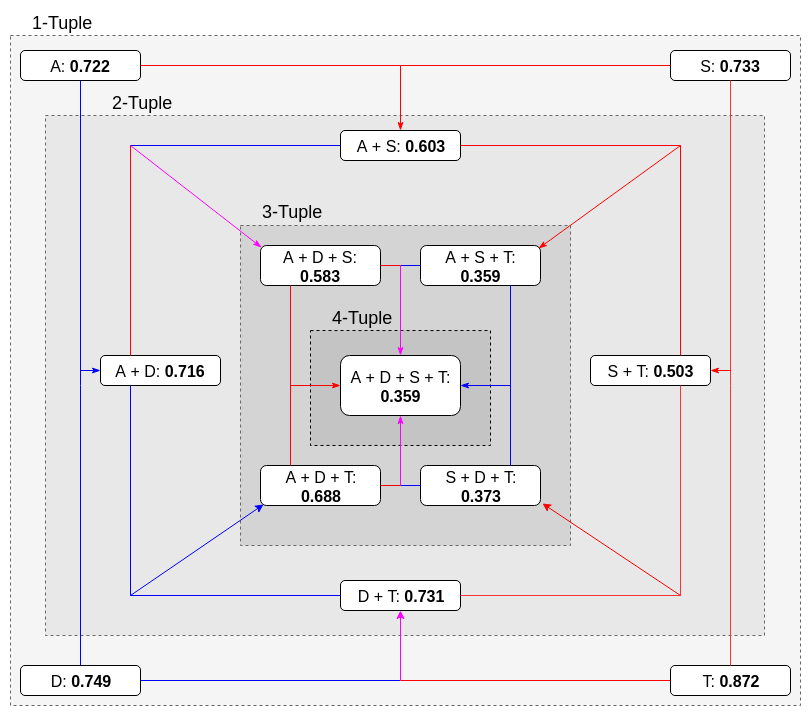
\includegraphics[width=.8\textwidth]{planar_combinations_v3}
	\caption{
		Target 10.0.0.100 Alert Dependency Graph
	}
	\label{fig:alert_depend_1}
\end{figure}

Stepping through the graph, nodes along the outer edges represent a single feature histogram. The values given are the histogram intersection between the ground truth and generated data distribution. As edges are traversed and meet, they are combined and arrive at the next node as a combination of the features considered. This process continues inwards, adding one more unique feature to each joint distribution, until all four features are considered at once.

It is important to note that for the 2-tuple combinations there are actually 6 possible distributions, however only 4 may be visualized while maintaining planarity of the graph; the analysis of these values is still included in the conditional and joint probability tables.

In order to highlight drops in intersection score, the following schema was applied to the graph: Lines are color coded such that blue lines indicate feature unions which result in less than 5\% difference between histogram scores. Conversely, lines which are red indicate an difference that is greater than 5\%. Lines which are purple indicate a unidirectional dependence relationship between the feature tuples. This occurs when one feature is a good predictor of another ($<$ 5\% intersection difference) but the opposite is not true ($>$ 5\% intersection difference). Lines which are blue or red exhibit bidirectional dependence; both lines exhibit the same intersection difference. All dashed lines are bounding boxes added to clearly segment the varying $m$-tuple histograms.

To verify that the graph correctly highlights feature dependencies Table \ref{tab:ce} was computed. This table considers all unique permutations of features for all m-tuple sizes across all 4 target IPs. The conditional entropy is then compared between the ground truth and generated data distributions. Additionally, the joint entropy was computed in Table \ref{tab:je} to provide a baselines representation of the amount of randomness in the feature distributions. This table contains calculations only from 2-tuple, 3-tuple, and 4-tuple combinations as there is no direct comparison to draw between conditional and joint entropy for single feature histograms.



\begin{table}[!htbp]
	\caption{Weighted Normalized Conditional Entropy Values for all Target IPs}
	\label{tab:ce}
	\centering
	\begin{adjustbox}{angle=90}
		\begin{tabular}{l|c|c|c|c|c|c|c|c|c|}
			\multicolumn{1}{c|}{} & \multicolumn{9}{c|}{\textbf{Victim Machine IP Address}} \\
			\multicolumn{1}{c|}{} & \multicolumn{4}{c|}{\textbf{Ground Truth Results}} &  & \multicolumn{4}{c|}{\textbf{Generated Results}} \\
			\multicolumn{1}{c|}{\textbf{Features}} & \textbf{10.0.0.100} & \textbf{10.0.0.27} & \textbf{10.0.0.22} & \textbf{10.0.99.143} &  & \textbf{10.0.0.100} & \textbf{10.0.0.27} & \textbf{10.0.0.22} & \textbf{10.0.99.143} \\ \cline{1-10}
			\multicolumn{1}{l|}{\textbf{A{\given}T}} & 0.556 & 0.452 & 0.695 & 0.434 &  & 0.020 & 0.570 & 0.003 & 0.561 \\
			\multicolumn{1}{l|}{\textbf{T{\given}S}} & 0.556 & 0.452 & 0.695 & 0.434 &  & 0.699 & 0.691 & 0.723 & 0.807 \\
			\multicolumn{1}{l|}{\textbf{T{\given}A}} & 0.660 & 0.621 & 0.735 & 0.575 &  & 0.725 & 0.810 & 0.778 & 0.658 \\
			\multicolumn{1}{l|}{\textbf{S{\given}T}} & 0.398 & 0.330 & 0.605 & 0.313 &  & 0.361 & 0.570 & 0.745 & 0.719 \\
			\multicolumn{1}{l|}{\textbf{S{\given}A}} & 0.800 & 0.752 & 0.831 & 0.711 &  & 0.397 & 0.727 & 0.836 & 0.625 \\
			\multicolumn{1}{l|}{\textbf{D{\given}S}} & 0.346 & 0.445 & 0.253 & 0.278 &  & 0.054 & 0.744 & 0.185 & 0.536 \\
			\multicolumn{1}{l|}{\textbf{A{\given}D}} & 0.080 & 0.222 & 0.070 & 0.288 &  & 0.025 & 0.536 & 0.004 & 0.564 \\
			\multicolumn{1}{l|}{\textbf{T{\given}D}} & 0.690 & 0.656 & 0.766 & 0.648 &  & 0.723 & 0.804 & 0.773 & 0.764 \\
			\multicolumn{1}{l|}{\textbf{D{\given}T}} & 0.260 & 0.406 & 0.185 & 0.219 &  & 0.052 & 0.743 & 0.200 & 0.516 \\
			\multicolumn{1}{l|}{\textbf{A{\given}S}} & 0.346 & 0.385 & 0.271 & 0.475 &  & 0.025 & 0.576 & 0.004 & 0.604 \\
			\multicolumn{1}{l|}{\textbf{S{\given}D}} & 0.822 & 0.779 & 0.856 & 0.785 &  & 0.392 & 0.715 & 0.821 & 0.698 \\
			\multicolumn{1}{l|}{\textbf{D{\given}A}} & 0.006 & 0.246 & 0.006 & 0.016 &  & 0.059 & 0.720 & 0.225 & 0.430 \\ \hline
			\multicolumn{1}{l|}{\textbf{S{\given}A,D}} & 0.799 & 0.747 & 0.829 & 0.705 &  & 0.389 & 0.762 & 0.812 & 0.334 \\
			\multicolumn{1}{l|}{\textbf{D{\given}S,T}} & 0.166 & 0.331 & 0.133 & 0.184 &  & 0.037 & 0.594 & 0.097 & 0.249 \\
			\multicolumn{1}{l|}{\textbf{S{\given}D,T}} & 0.229 & 0.191 & 0.516 & 0.255 &  & 0.353 & 0.578 & 0.718 & 0.395 \\
			\multicolumn{1}{l|}{\textbf{T{\given}A,D}} & 0.657 & 0.613 & 0.733 & 0.568 &  & 0.725 & 0.848 & 0.784 & 0.351 \\
			\multicolumn{1}{l|}{\textbf{A{\given}S,D}} & 0.069 & 0.206 & 0.056 & 0.245 &  & 0.024 & 0.542 & 0.007 & 0.311 \\
			\multicolumn{1}{l|}{\textbf{A{\given}S,T}} & 0.174 & 0.259 & 0.142 & 0.350 &  & 0.016 & 0.553 & 0.006 & 0.262 \\
			\multicolumn{1}{l|}{\textbf{A{\given}D,T}} & 0.050 & 0.183 & 0.037 & 0.212 &  & 0.019 & 0.523 & 0.006 & 0.273 \\
			\multicolumn{1}{l|}{\textbf{D{\given}A,S}} & 0.005 & 0.243 & 0.005 & 0.012 &  & 0.050 & 0.594 & 0.116 & 0.198 \\
			\multicolumn{1}{l|}{\textbf{T{\given}S,D}} & 0.393 & 0.340 & 0.587 & 0.348 &  & 0.697 & 0.716 & 0.726 & 0.463 \\
			\multicolumn{1}{l|}{\textbf{D{\given}A,T}} & 0.004 & 0.238 & 0.003 & 0.007 &  & 0.050 & 0.585 & 0.117 & 0.171 \\
			\multicolumn{1}{l|}{\textbf{S{\given}A,T}} & 0.211 & 0.178 & 0.500 & 0.228 &  & 0.362 & 0.592 & 0.730 & 0.279 \\
			\multicolumn{1}{l|}{\textbf{T{\given}A,S}} & 0.365 & 0.312 & 0.561 & 0.302 &  & 0.701 & 0.723 & 0.733 & 0.332 \\ \hline
			\multicolumn{1}{l|}{\textbf{A{\given}S,D,T}} & 0.041 & 0.172 & 0.028 & 0.195 &  & 0.009 & 0.494 & 0.003 & 0.103 \\
			\multicolumn{1}{l|}{\textbf{D{\given}A,S,T}} & 0.002 & 0.232 & 0.002 & 0.004 &  & 0.038 & 0.556 & 0.082 & 0.063 \\
			\multicolumn{1}{l|}{\textbf{S{\given}A,D,S}} & 0.209 & 0.167 & 0.498 & 0.222 &  & 0.330 & 0.572 & 0.720 & 0.137 \\
			\multicolumn{1}{l|}{\textbf{T{\given}A,S,D}} & 0.362 & 0.302 & 0.558 & 0.294 &  & 0.688 & 0.643 & 0.732 & 0.160
		\end{tabular}
	\end{adjustbox}
\end{table}

\begin{table}[!htbp]
	\caption{Normalized Joint Entropy Values for all Victim IPs}
	\label{tab:je}
	\centering
	\begin{adjustbox}{angle=90}
		\begin{tabular}{l|c|c|c|c|c|c|c|c|c|}
			\multicolumn{1}{c|}{} & \multicolumn{9}{c|}{\textbf{Victim Machine IP Address}} \\
			\multicolumn{1}{c|}{} & \multicolumn{4}{c|}{\textbf{Ground Truth Results}} &  & \multicolumn{4}{c|}{\textbf{Generated Results}} \\
			\multicolumn{1}{c|}{\textbf{Features}} & \textbf{10.0.0.100} & \textbf{10.0.0.27} & \textbf{10.0.0.22} & \textbf{10.0.99.143} & \textbf{} & \textbf{10.0.0.100} & \textbf{10.0.0.27} & \textbf{10.0.0.22} & \textbf{10.0.99.143} \\ \hline
			\textbf{A+T} & 0.655 & 0.691 & 0.675 & 0.700 &  & 0.664 & 0.788 & 0.783 & 0.887 \\
			\textbf{A+S} & 0.597 & 0.633 & 0.566 & 0.712 &  & 0.347 & 0.713 & 0.826 & 0.867 \\
			\textbf{S+D} & 0.613 & 0.680 & 0.551 & 0.580 &  & 0.349 & 0.767 & 0.699 & 0.792 \\
			\textbf{D+T} & 0.671 & 0.742 & 0.684 & 0.613 &  & 0.630 & 0.803 & 0.715 & 0.823 \\
			\textbf{S+T} & 0.763 & 0.714 & 0.874 & 0.728 &  & 0.729 & 0.793 & 0.817 & 0.899 \\
			\textbf{A+D} & 0.373 & 0.591 & 0.302 & 0.522 &  & 0.078 & 0.626 & 0.214 & 0.812 \\ \hline
			\textbf{A+S+T} & 0.682 & 0.708 & 0.776 & 0.728 &  & 0.718 & 0.808 & 0.817 & 0.959 \\
			\textbf{A+S+D} & 0.591 & 0.745 & 0.554 & 0.696 &  & 0.337 & 0.765 & 0.699 & 0.922 \\
			\textbf{A+D+T} & 0.652 & 0.799 & 0.670 & 0.695 &  & 0.607 & 0.808 & 0.715 & 0.934 \\
			\textbf{S+D+T} & 0.692 & 0.752 & 0.784 & 0.651 &  & 0.708 & 0.811 & 0.807 & 0.940 \\ \hline
			\textbf{A+S+D+T} & 0.681 & 0.808 & 0.774 & 0.726 &  & 0.702 & 0.833 & 0.807 & 0.974 \\
		\end{tabular}
	\end{adjustbox}
\end{table}

Several instances of feature dependency show good agreement between Fig. \ref{fig:alert_depend_1} and Table \ref{tab:ce}. To draw this conclusion it is important to consider that the conditional entropy of the generated data and ground truth distribution are similar and low in magnitude.

To further study specific feature-value relationships between the ground truth and generated data distributions complete probability tables may be output for each feature permutation. In order to make this tables human-readable the following color schema is applied: cells which have probability 0 are highlighted in red; cells with probability 1 are highlighted in green. This two step process highlights both the sparsity of output probabilities as well as cases where the input results in a deterministic output.

Further exploring the feature dependency agreement between X and Y, the conditional probability tables for both the ground truth and generated distribution are reviewed. Fig. \ref{fig:feat_depend_tab} shows some of the specific feature values that results in the conditional entropy values noted. Note that the output value Y is very deterministic once a specific input X is given.



\subsection{WGAN-GPMI Feature Dependency Performance}

All of the aforementioned plots and tables were created in duplicate in order to test the effect of Mutual Information maximization on the model's ability to capture feature dependencies.

First, the graph structure and highlighting in Fig. \ref{fig:alert_depend_1} was applied to the histogram intersection scores of the WGAN-GPMI model in Fig. \ref{fig:alert_depend_5}. Similar to the WGAN-GP model results, Appendix \ref{sec:depend_app} contains the results for the other three target IP addresses tested. Note that from this figure alone it is impossible to make a claim that feature dependencies are more fully captured by the WGAN-GPMI model. However by computing the conditional entropy in Table \ref{tab:ce2} it is apparent that the WGAN-GPMI model more closely imitates the entropy of the ground truth.

\begin{figure}[!htbp]
	\centering
	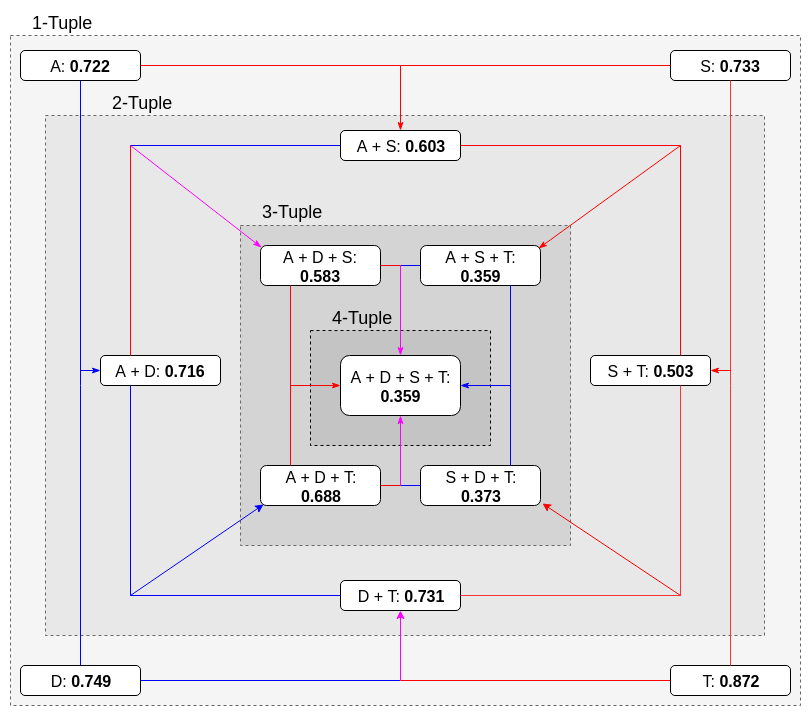
\includegraphics[width=.8\textwidth]{planar_combinations_v3}
	\caption{
		Target 10.0.0.100 Alert Dependency Graph
	}
	\label{fig:alert_depend_5}
\end{figure}


\begin{table}[!htbp]
	\caption{Weighted Normalized Conditional Entropy Values for all Target IPs}
	\label{tab:ce2}
	\centering
	\begin{adjustbox}{angle=90}
		\begin{tabular}{l|c|c|c|c|c|c|c|c|c|}
			\multicolumn{1}{c|}{} & \multicolumn{9}{c|}{\textbf{Victim Machine IP Address}} \\
			\multicolumn{1}{c|}{} & \multicolumn{4}{c|}{\textbf{Ground Truth Results}} &  & \multicolumn{4}{c|}{\textbf{Generated Results}} \\
			\multicolumn{1}{c|}{\textbf{Features}} & \textbf{10.0.0.100} & \textbf{10.0.0.27} & \textbf{10.0.0.22} & \textbf{10.0.99.143} &  & \textbf{10.0.0.100} & \textbf{10.0.0.27} & \textbf{10.0.0.22} & \textbf{10.0.99.143} \\ \cline{1-10}
			\multicolumn{1}{l|}{\textbf{A{\given}T}} & 0.556 & 0.452 & 0.695 & 0.434 &  & 0.020 & 0.570 & 0.003 & 0.561 \\
			\multicolumn{1}{l|}{\textbf{T{\given}S}} & 0.556 & 0.452 & 0.695 & 0.434 &  & 0.699 & 0.691 & 0.723 & 0.807 \\
			\multicolumn{1}{l|}{\textbf{T{\given}A}} & 0.660 & 0.621 & 0.735 & 0.575 &  & 0.725 & 0.810 & 0.778 & 0.658 \\
			\multicolumn{1}{l|}{\textbf{S{\given}T}} & 0.398 & 0.330 & 0.605 & 0.313 &  & 0.361 & 0.570 & 0.745 & 0.719 \\
			\multicolumn{1}{l|}{\textbf{S{\given}A}} & 0.800 & 0.752 & 0.831 & 0.711 &  & 0.397 & 0.727 & 0.836 & 0.625 \\
			\multicolumn{1}{l|}{\textbf{D{\given}S}} & 0.346 & 0.445 & 0.253 & 0.278 &  & 0.054 & 0.744 & 0.185 & 0.536 \\
			\multicolumn{1}{l|}{\textbf{A{\given}D}} & 0.080 & 0.222 & 0.070 & 0.288 &  & 0.025 & 0.536 & 0.004 & 0.564 \\
			\multicolumn{1}{l|}{\textbf{T{\given}D}} & 0.690 & 0.656 & 0.766 & 0.648 &  & 0.723 & 0.804 & 0.773 & 0.764 \\
			\multicolumn{1}{l|}{\textbf{D{\given}T}} & 0.260 & 0.406 & 0.185 & 0.219 &  & 0.052 & 0.743 & 0.200 & 0.516 \\
			\multicolumn{1}{l|}{\textbf{A{\given}S}} & 0.346 & 0.385 & 0.271 & 0.475 &  & 0.025 & 0.576 & 0.004 & 0.604 \\
			\multicolumn{1}{l|}{\textbf{S{\given}D}} & 0.822 & 0.779 & 0.856 & 0.785 &  & 0.392 & 0.715 & 0.821 & 0.698 \\
			\multicolumn{1}{l|}{\textbf{D{\given}A}} & 0.006 & 0.246 & 0.006 & 0.016 &  & 0.059 & 0.720 & 0.225 & 0.430 \\ \hline
			\multicolumn{1}{l|}{\textbf{S{\given}A,D}} & 0.799 & 0.747 & 0.829 & 0.705 &  & 0.389 & 0.762 & 0.812 & 0.334 \\
			\multicolumn{1}{l|}{\textbf{D{\given}S,T}} & 0.166 & 0.331 & 0.133 & 0.184 &  & 0.037 & 0.594 & 0.097 & 0.249 \\
			\multicolumn{1}{l|}{\textbf{S{\given}D,T}} & 0.229 & 0.191 & 0.516 & 0.255 &  & 0.353 & 0.578 & 0.718 & 0.395 \\
			\multicolumn{1}{l|}{\textbf{T{\given}A,D}} & 0.657 & 0.613 & 0.733 & 0.568 &  & 0.725 & 0.848 & 0.784 & 0.351 \\
			\multicolumn{1}{l|}{\textbf{A{\given}S,D}} & 0.069 & 0.206 & 0.056 & 0.245 &  & 0.024 & 0.542 & 0.007 & 0.311 \\
			\multicolumn{1}{l|}{\textbf{A{\given}S,T}} & 0.174 & 0.259 & 0.142 & 0.350 &  & 0.016 & 0.553 & 0.006 & 0.262 \\
			\multicolumn{1}{l|}{\textbf{A{\given}D,T}} & 0.050 & 0.183 & 0.037 & 0.212 &  & 0.019 & 0.523 & 0.006 & 0.273 \\
			\multicolumn{1}{l|}{\textbf{D{\given}A,S}} & 0.005 & 0.243 & 0.005 & 0.012 &  & 0.050 & 0.594 & 0.116 & 0.198 \\
			\multicolumn{1}{l|}{\textbf{T{\given}S,D}} & 0.393 & 0.340 & 0.587 & 0.348 &  & 0.697 & 0.716 & 0.726 & 0.463 \\
			\multicolumn{1}{l|}{\textbf{D{\given}A,T}} & 0.004 & 0.238 & 0.003 & 0.007 &  & 0.050 & 0.585 & 0.117 & 0.171 \\
			\multicolumn{1}{l|}{\textbf{S{\given}A,T}} & 0.211 & 0.178 & 0.500 & 0.228 &  & 0.362 & 0.592 & 0.730 & 0.279 \\
			\multicolumn{1}{l|}{\textbf{T{\given}A,S}} & 0.365 & 0.312 & 0.561 & 0.302 &  & 0.701 & 0.723 & 0.733 & 0.332 \\ \hline
			\multicolumn{1}{l|}{\textbf{A{\given}S,D,T}} & 0.041 & 0.172 & 0.028 & 0.195 &  & 0.009 & 0.494 & 0.003 & 0.103 \\
			\multicolumn{1}{l|}{\textbf{D{\given}A,S,T}} & 0.002 & 0.232 & 0.002 & 0.004 &  & 0.038 & 0.556 & 0.082 & 0.063 \\
			\multicolumn{1}{l|}{\textbf{S{\given}A,D,S}} & 0.209 & 0.167 & 0.498 & 0.222 &  & 0.330 & 0.572 & 0.720 & 0.137 \\
			\multicolumn{1}{l|}{\textbf{T{\given}A,S,D}} & 0.362 & 0.302 & 0.558 & 0.294 &  & 0.688 & 0.643 & 0.732 & 0.160
		\end{tabular}
	\end{adjustbox}
\end{table}

\section{Output Modes Captured}
\label{sec:output}
Finally, to assess output modes captured by each model, two values were collected; the number of values that existed in the ground truth that were not generated by the model and the number of values generated by the model that never occurred in the ground truth. Like all previous metrics, these values were collected for each unique m-tuple combination of features. Table \ref{tab:output_modes} shows the number of output modes missed by the generative model. Note that this table shows the direct benefit of mutual information maximization, as the number of output modes missed by the model decreases across the board for the WGAN-GPMI model.

Table \ref{tab:random_outputs} shows the number of noisy outputs by the generative model  that did not occur in the ground truth. These results are less clear cut. For target IP 10.0.99.143, the target IP tested with the lowest number of alerts, the WGAN-GPMI model appears to create less noisy outputs. However, for other IPs such as 10.0.0.100, the models perform comparably.

\begin{table}[!htbp]
	\centering
	\caption{Noisy Generator Output Counts}
	\label{tab:random_outputs}
	\begin{adjustbox}{angle=90}
		\begin{tabular}{c|c|c|c|c|c|c|c|c}
			\multicolumn{1}{l|}{} & \multicolumn{4}{l|}{\textbf{Target IP Address (WGAN-GP)}} & \multicolumn{4}{l}{\textbf{Target IP Address (WGAN-GPMI)}} \\ \hline

			\textbf{M} & \multicolumn{1}{l|}{\textbf{10.0.0.100}} & \multicolumn{1}{l|}{\textbf{10.0.0.27}} & \multicolumn{1}{l|}{\textbf{10.0.0.22}} & \multicolumn{1}{l|}{\textbf{10.0.99.143}} & \multicolumn{1}{l|}{\textbf{10.0.0.100}} & \multicolumn{1}{l|}{\textbf{10.0.0.27}} & \multicolumn{1}{l|}{\textbf{10.0.0.22}} & \multicolumn{1}{l}{\textbf{10.0.99.143}} \\
			\hline
			\textbf{4} & 168 & 235 & 76 & 321 & 213 & 97 & 107 & 98 \\
			\hline 
			\multirow{4}{*}{\textbf{3}} & 131 & 112 & 46 & 192 & 103 & 60 & 63 & 50 \\
			& 119 & 97 & 36  & 240 & 83 & 40 & 34 & 40 \\
			& 49  & 23 & 6  & 187  & 117 & 57  & 52 & 57 \\
			& 54  & 46 & 17 & 174  & 84  & 57  & 68 & 40 \\
			\hline
			\multirow{6}{*}{\textbf{2}} & 70 & 23 & 29 & 95 & 31 & 23 & 13 & 20 \\
			& 22  & 0 & 0  & 60 & 11 & 12 & 12 & 4  \\
			& 12  & 1 & 1  & 68 & 39 & 24 & 12 & 21 \\
			& 10  & 9 & 3  & 71 & 20 & 14 & 11 & 8  \\
			& 20  & 5 & 1  & 94 & 14 & 16 & 26 & 3  \\
			& 19  & 2 & 1  & 58 & 23 & 20 & 22 & 10 \\
			\hline
			\multirow{4}{*}{\textbf{1}} & 0  & 0  & 0  & 5  & 0  & 0  & 0  & 0  \\
			& 2   & 0 & 0  & 24 & 0  & 0  & 0  & 0  \\
			& 11  & 0 & 0  & 17 & 0  & 0  & 0  & 0  \\
			& 0   & 0 & 0  & 30 & 0  & 0  & 0  & 1  \\
			\hline
			\multicolumn{1}{l|}{\textbf{\# Combinations}} & 286200 & 185976 & 128520 & 189658 & \multicolumn{1}{l|}{} & \multicolumn{1}{l|}{} & \multicolumn{1}{l|}{} & \multicolumn{1}{l}{}
		\end{tabular}
	\end{adjustbox}
\end{table}
